\section{平面二次曲线及其方程}
\subsection{圆}
\subsubsection{圆的概念与方程}
\begin{definition}
平面内与定点距离等于定长的点的集合是\DefineConcept{圆}.定点称为\DefineConcept{圆心},定长称为\DefineConcept{半径}.
\end{definition}

根据圆的定义,我们来求圆心是\(C(a,b)\),半径是\(r\)的圆的方程.
设点\(P(x,y)\)是圆上任意一点,根据定义,点\(P\)到圆心\(C\)的距离等于\(r\).圆就是点集\begin{equation*}
	\Set{ P \given \abs{PC} = r }.
\end{equation*}
由两点间的距离公式,\begin{equation*}
	\abs{PC} = \sqrt{(x-a)^2+(y-b)^2} = r.
\end{equation*}
把上式等号两边分别平方,得\begin{equation}
	(x-a)^2+(y-b)^2 = r^2.
\end{equation}上面这个方程式就是圆心是\(C(a,b)\),半径是\(r\)的圆的方程,我们称之为\DefineConcept{圆的标准方程}.
特别地,如果圆心在坐标原点,即\(a=b=0\)时,那么圆的方程就是\begin{equation}
x^2+y^2 = r^2.
\end{equation}

把圆的标准方程\begin{equation*}
	(x-a)^2+(y-b)^2 = r^2
\end{equation*}
展开,得\begin{equation*}
	x^2 + y^2 - 2ax - 2by + a^2 + b^2 - r^2 = 0.
\end{equation*}
可见,任何一个圆的方程都可以写成下面的形式\begin{equation*}
	x^2 + y^2 + Dx + Ey + F = 0.
\end{equation*}
反过来,我们来研究上式确定的曲线是不是圆,将其配方,得\begin{equation*}
\left(x+\frac{D}{2}\right)^2+\left(y+\frac{E}{2}\right)^2 = \frac{D^2+E^2-4F}{4}.
\end{equation*}\begin{enumerate}
	\item 当\(D^2+E^2-4F > 0\)时,
	比较上式与圆的标准方程,可知上述曲线是以\((-\frac{D}{2},-\frac{E}{2})\)为圆心、
	\(\frac{1}{2} \sqrt{D^2+E^2-4F}\)为半径的圆;

	\item 当\(D^2+E^2-4F = 0\)时,
	上式只有实数解\(x=-\frac{D}{2}\),\(y=-\frac{E}{2}\),
	所以上述曲线是一个点\((-\frac{D}{2},-\frac{E}{2})\);

	\item 当\(D^2+E^2-4F < 0\)时,
	上式没有实数解,因而它不表示任何图形.
\end{enumerate}
综上所述,方程\begin{equation}
	x^2 + y^2 + Dx + Ey + F = 0,
	\quad
	D^2+E^2-4F > 0
\end{equation}
表示一个圆,叫做\DefineConcept{圆的一般方程}.

方程\begin{equation}
	\left\{ \begin{array}{l}
		x = a + r \cos\theta, \\
		y = b + r \sin\theta
	\end{array} \right.
\end{equation}
表示以\((a,b)\)为圆心、\(r\)为半径的圆,
叫做\DefineConcept{圆的参数方程}.

圆的标准方程的优点在于它明确地指出了圆心和半径,
而一般方程突出了方程形式上的特点:\begin{enumerate}
	\item \(x^2\)和\(y^2\)的系数相同,且均不为零;
	\item 没有\(xy\)这样的二次项.
\end{enumerate}
以上两点是二元二次方程\begin{equation*}
	A x^2 + B xy + C y^2 + D x + E y + F = 0
\end{equation*}表示圆的必要不充分条件.

\subsubsection{圆与点的位置关系}
已知圆\(C: (x-a)^2+(y-b)^2=r^2\).
任给一点\(P(x_0,y_0)\),令\(z_0 = (x_0-a)^2+(y_0-b)^2\).
若\(z_0 < r^2\),则称点\(P\)在圆\(C\)的内部;
若\(z_0 = r^2\),则称点\(P\)在圆\(C\)上;
若\(z_0 > r^2\),则称点\(P\)在圆\(C\)的外部.

若圆\(C\)的方程是\(x^2+y^2+Dx+Ey+F=0\),则令\(u_0 = x_0^2+y_0^2+Dx_0+Ey_0+F\).
只要\(u_0 < 0\),则称点\(P\)在圆\(C\)内;
只要\(u_0 = 0\),则称点\(P\)在圆\(C\)上;
只要\(u_0 > 0\),则称点\(P\)在圆\(C\)外.

\subsubsection{圆与直线的位置关系}
\begin{example}
已知圆的方程是\(x^2+y^2 = r^2\),求经过圆上一点\(P(x_0,y_0)\)的切线的方程.
\begin{solution}
设切线的斜率为\(k\),半径\(OP\)的斜率为\(k_1\).因为圆的切线垂直于过切点的半径,于是\(k = -\frac{1}{k_1}\).又因为\(k_1 = \frac{y_0}{x_0}\),所以\(k = -\frac{x_0}{y_0}\),那么经过点\(P\)的切线方程是\begin{equation*}
y-y_0 = -\frac{x_0}{y_0} (x-x_0),
\end{equation*}整理得\begin{equation*}
x_0 x + y_0 y = x_0^2 + y_0^2.
\end{equation*}因为\(P(x_0,y_0)\)在圆上,所以\(x_0^2 + y_0^2 = r^2\),所求切线方程是\begin{equation}
x_0 x + y_0 y = r^2.
\end{equation}
\end{solution}
\end{example}

\begin{example}
已知平面直线\(l: x + y = a\)与圆\(C: x^2 + y^2 = r^2\).
求当直线\(l\)与圆\(C\)相交、相切或相离时,参数\(a\)与\(r\)的关系.
\end{example}

\subsubsection{圆与圆的位置关系}
已知两个圆:\begin{equation*}
	(x-x_1)^2+(y-y_1)^2=R^2
	\quad\text{和}\quad
	(x-x_2)^2+(y-y_2)^2=r^2,
\end{equation*}其中\(R \geq r\).
设两圆的圆心距为\(d\).
记方程组\begin{equation*}
	M: \begin{cases}
		(x-x_1)^2+(y-y_1)^2=R^2, \\
		(x-x_2)^2+(y-y_2)^2=r^2.
	\end{cases}
\end{equation*}

\begin{table}[htb]
	\centering
	\begin{tblr}{*3c}
		\hline
		位置关系 & 几何特征 & 代数特征 \\ \hline
		外离 & \(d>R+r\) & \(M\)无实数解 \\
		外切 & \(d=R+r\) & \(M\)有一组实数解 \\
		相交 & \(R-r<d<R+r\) & \(M\)有两组实数解 \\
		内切 & \(d=R-r\) & \(M\)有一组实数解 \\
		内含 & \(d<R-r\) & \(M\)无实数解 \\
		\hline
	\end{tblr}
	\caption{圆与圆的位置关系}
\end{table}

\subsubsection{圆系的方程}
%@see: https://www.bilibili.com/video/BV1UuChYJE1d/
假设有两个不重合的定点\(P_1(x_1,y_1)\)和\(P_2(x_2,y_2)\).
我们想求出经过这两个点的所有的圆的方程.
设某个圆的方程为\begin{equation*}
	x^2 + y^2 + Cx + Dy + E = 0.
\end{equation*}
依次代入\(P_1,P_2\)两点的坐标,得\begin{gather*}
	x_1 C + y_1 D + E = -(x_1^2 + y_1^2), \\
	x_2 C + y_2 D + E = -(x_2^2 + y_2^2),
\end{gather*}
或者\begin{equation}\label{equation:解析几何.过不重合两点的圆系方程}
	\begin{bmatrix}
		x_1 & y_1 & 1 \\
		x_2 & y_2 & 1
	\end{bmatrix}
	\begin{bmatrix}
		C \\ D \\ E
	\end{bmatrix}
	= \begin{bmatrix}
		-(x_1^2 + y_1^2) \\
		-(x_2^2 + y_2^2)
	\end{bmatrix}.
\end{equation}
由于\(P_1,P_2\)不重合,
\((x_1,y_1) \neq (x_2,y_2)\),
所以\((x_1,y_1,1),(x_2,y_2,1)\)线性无关,
从而有\begin{equation*}
	\rank\begin{bmatrix}
		x_1 & y_1 & 1 \\
		x_2 & y_2 & 1
	\end{bmatrix}
	= \rank\begin{bmatrix}
		x_1 & y_1 & 1 & -(x_1^2 + y_1^2) \\
		x_2 & y_2 & 1 & -(x_2^2 + y_2^2)
	\end{bmatrix}
	= 2 < 3.
\end{equation*}
方程 \labelcref{equation:解析几何.过不重合两点的圆系方程} 有无穷多解,
它的解空间是\(1\)维的,
其中每一个解都确定了一个圆.
不妨设方程 \labelcref{equation:解析几何.过不重合两点的圆系方程} 的通解为\begin{equation*}
	(C,D,E)^T
	= (C_0,D_0,E_0)^T
	+ \lambda (C_1,D_1,E_1)^T,
\end{equation*}
其中\(\lambda\)是任意常数.
那么过\(P_1(x_1,y_1),P_2(x_2,y_2)\)两点的圆系方程为\begin{equation*}
	x^2 + y^2 + C_0 x + D_0 y + E_0 + \lambda (C_1 x + D_1 y + E_1) = 0.
\end{equation*}
可以注意到,
\((C_0,D_0,E_0)^T\)是非齐次方程\begin{equation*}
	\begin{cases}
		x_1 C + y_1 D + E = -(x_1^2 + y_1^2), \\
		x_2 C + y_2 D + E = -(x_2^2 + y_2^2)
	\end{cases}
\end{equation*}
的一个解,
而\((C_1,D_1,E_1)^T\)是齐次方程\begin{equation*}
	\begin{cases}
		x_1 C + y_1 D + E = 0, \\
		x_2 C + y_2 D + E = 0
	\end{cases}
\end{equation*}
的解(或者说\((C_1,D_1,E_1)^T\)是由\(P_1(x_1,y_1),P_2(x_2,y_2)\)两点确定的直线的方程的参数).

\subsection{椭圆}
\begin{definition}
平面内与两个定点的距离之和等于定长的点的集合是\DefineConcept{椭圆}(ellipse).
这两个定点叫做椭圆的\DefineConcept{焦点}(focus).
两焦点的距离叫做\DefineConcept{焦距}.
\end{definition}

根据椭圆的定义,我们来求椭圆的方程.
取过焦点\(F_1\)、\(F_2\)的直线为\(x\)轴,
线段\(F_1 F_2\)的垂直平分线为\(y\)轴,
建立直角坐标系.

设\(P(x,y)\)是椭圆上任意一点,椭圆的焦距为\(2c\ (c > 0)\),
\(P\)与\(F_1\)和\(F_2\)的距离之和等于正常数\(2a\),
则\(F_1\)、\(F_2\)的坐标分别是\((-c,0)\)和\((c,0)\).
那么根据定义,椭圆就是点集\begin{equation*}
	\Set{ P \given \abs{P F_1} + \abs{P F_2} = 2a }.
\end{equation*}
由两点间的距离公式,\begin{equation*}
	\abs{P F_1} = \sqrt{(x+c)^2+y^2}, \qquad
	\abs{P F_2} = \sqrt{(x-c)^2+y^2},
\end{equation*}得\begin{equation*}
	\sqrt{(x+c)^2+y^2} + \sqrt{(x-c)^2+y^2} = 2a,
\end{equation*}
把这个方程移项,两边平方,得\begin{equation*}
	(x+c)^2+y^2 = 4a^2 - 4a\sqrt{(x-c)^2+y^2} + (x-c)^2+y^2,
\end{equation*}\begin{equation*}
	a^2 - cx = a\sqrt{(x-c)^2+y^2},
\end{equation*}两边再平方,得\begin{equation*}
	a^4 - 2 a^2 cx + c^2 x^2 = a^2 [(x-c)^2+y^2],
\end{equation*}整理得\begin{equation*}
	(a^2 - c^2) x^2 + a^2 y^2 = a^2 (a^2 - c^2).
\end{equation*}由椭圆定义可知,\(2a > 2c\),\(a > c\),\(a^2 - c^2 > 0\).
设\(b^2 = a^2 - c^2\ (b > 0)\),得\begin{equation*}
	b^2 x^2 + a^2 y^2 = a^2 b^2,
\end{equation*}
两边除以\(a^2 b^2\),得\begin{equation}\label{equation:解析几何.椭圆的标准方程1}
	\frac{x^2}{a^2} + \frac{y^2}{b^2} = 1,
	\quad a > b > 0.
\end{equation}
方程 \labelcref{equation:解析几何.椭圆的标准方程1} 叫做\DefineConcept{椭圆的标准方程}.
它所表示的椭圆的焦点在\(x\)轴上,
焦点是\(F_1(-c,0)\)和\(F_2(c,0)\),
其中\(c^2 = a^2 - b^2\).

如果椭圆的焦点在\(y\)轴上,焦点是\(F_1(0,-c)\)和\(F_2(0,c)\),
只要将方程 \labelcref{equation:解析几何.椭圆的标准方程1} 中的\(x\)、\(y\)互换,就可以得到它的方程.
这时它的方程为\begin{equation}\label{equation:解析几何.椭圆的标准方程2}
	\frac{y^2}{a^2} + \frac{x^2}{b^2} = 1,
	\quad a > b > 0.
\end{equation}
方程 \labelcref{equation:解析几何.椭圆的标准方程2} 也是椭圆的标准方程.

\begin{figure}[htb]
	\centering
	\begin{tikzpicture}
		%\draw[gray,help lines,dashed] (-5,-3) grid (5,3);
		\draw[thick,->] (-6,0) -- (7,0)node[above]{\(x\)};
		\draw[thick,->] (0,-4) -- (0,4)node[right]{\(y\)};
		\pgfmathsetmacro{\a}{5}
		\pgfmathsetmacro{\b}{3}
		\pgfmathsetmacro{\c}{sqrt(\a*\a-\b*\b)}
		\pgfmathsetmacro{\px}{3}
		\pgfmathsetmacro{\py}{12/5}
		\pgfmathsetmacro{\dx}{\a*\a/\c}  % directrix
		\coordinate (P) at (\px,\py);
		\coordinate (Q) at (\dx,\py);
		\coordinate (R) at (\dx,0);
		\coordinate (M) at (\c,9/5);
		\coordinate (N) at (\c,-9/5);
		\coordinate (F1) at (-\c,0);
		\coordinate (F2) at (\c,0);
		\draw[orange] (0,0)ellipse[x radius=\a,y radius=\b];
		\draw[red] (F1)node[below right,black]{\(F_1\)}
			-- (P)node[above right,black]{\(P\)}
			-- (F2)node[below left,black]{\(F_2\)}
			(P) -- (Q)node[right,black]{\(Q\)}
			pic[draw=gray,-,angle radius=0.3cm]{right angle=P--Q--R}
			pic[draw=gray,-,angle radius=0.3cm]{right angle=N--F2--R};
		\draw[blue] (N)node[right,black]{\(N\)}
			-- (M)node[right,black]{\(M\)};
		\draw[purple] (\dx,-4) -- (\dx,4);
		\draw (-3,2)node[above left]{\(C: \frac{x^2}{a^2}+\frac{y^2}{b^2}=1\)}
			(\dx,-3)node[left]{\(l: x = \frac{a^2}{c}\)};
		\draw (0,0)node[below left]{\(O\)}
			(-5,0)node[above left]{\(A_1\)}
			(5,0)node[above right]{\(A_2\)}
			(0,-3)node[below right]{\(B_1\)}
			(0,3)node[above right]{\(B_2\)};
	\end{tikzpicture}
	\caption{椭圆的图形}
	\label{figure:解析几何.椭圆的图形}
\end{figure}

我们根据椭圆的标准方程\begin{equation*}
	\frac{x^2}{a^2} + \frac{y^2}{b^2} = 1,
	\quad a > b > 0
\end{equation*}来研究椭圆的几何性质.
\begin{enumerate}
\item 范围

由标准方程可知,椭圆上点的坐标\((x,y)\)都适合不等式\begin{equation*}
\frac{x^2}{a^2} \leq 1, \qquad \frac{y^2}{b^2} \leq 1,
\end{equation*}即\begin{equation*}
x^2 \leq a^2, \qquad y^2 \leq b^2,
\end{equation*}\begin{equation*}
\abs{x} \leq a, \qquad \abs{y} \leq b.
\end{equation*}这说明椭圆位于直线\(x=\pm a\)和\(y=\pm b\)所围成的矩形里.

\item 对称性

在标准方程中,把\(x\)换成\(-x\),或把\(y\)换成\(-y\),或把\(x\)、\(y\)同时换成\(-x\)、\(-y\)时,
方程都不变,所以图形关于\(y\)轴、\(x\)轴和原点都是对称的.
也就是说,坐标轴是椭圆的对称轴,原点是椭圆的对称中心.
椭圆的对称中心叫做椭圆的\DefineConcept{中心}.

\item 顶点

在标注方程中,令\(x=0\),得\(y=\pm b\),
这说明\(B_1(0,-b)\)和\(B_2(0,b)\)是椭圆和\(y\)轴的两个交点.
同理,令\(y=0\),得\(x=\pm a\),
说明\(A_1(-a,0)\)和\(A_2(a,0)\)是椭圆和\(x\)轴的两个交点.
因为\(x\)轴和\(y\)轴是椭圆的对称轴,所以椭圆和它的对称轴共有四个交点.
这四个交点叫做椭圆的\DefineConcept{顶点}.

线段\(A_1 A_2\)和\(B_1 B_2\)分别叫做%
椭圆的\DefineConcept{长轴}(major axis)%
和\DefineConcept{短轴}(minor axis).
它们的长为\begin{equation*}
\abs{A_1 A_2} = 2a, \qquad \abs{B_1 B_2} = 2b.
\end{equation*}而\(a\)和\(b\)分别叫做椭圆的长半轴长和短半轴长.

\item 离心率

椭圆的焦距与长轴长的比\(e = \frac{c}{a}\)叫做椭圆的\DefineConcept{离心率}(eccentricity).
因为\(a > c > 0\),所以\(0 < e < 1\).

\(e\)越接近\(1\),则\(c\)越接近\(a\),从而\(b = \sqrt{a^2 - c^2}\)越小,因此椭圆越扁;
反之,\(e\)越接近\(0\),\(c\)越接近\(0\),从而\(b\)越接近\(a\),这时椭圆就接近于圆.
如果\(a=b\),则\(c=0\),两个焦点重合,这时椭圆的标准方程成为\begin{equation*}
x^2 + y^2 = a^2,
\end{equation*}
它的图形就是圆了;
因此可以把圆\(x^2+y^2=a^2\)看作离心率为\(0\)的椭圆.
\end{enumerate}

\begin{example}
我国于1970年4月24日发射的第一颗人造地球卫星(东方红一号卫星)的运行轨道,是以地球的重心为一个焦点的椭圆,近地点\(A\)距离地面439公里,远地点\(B\)距离地面2384公里,地球半径约为6371公里.求卫星的轨道方程.
\begin{solution}
由题可知\begin{equation*}
a - c = 6371 + 439 = 6810,
\end{equation*}\begin{equation*}
a + c = 6371 + 2384 = 8755.
\end{equation*}解得\(a=7782.5\),\(c=972.5\),所以\(b=\sqrt{a^2-c^2}=\sqrt{(a+c)(a-c)}=7721.5\).因此,卫星的轨道方程是\begin{equation*}
\frac{x^2}{7783^2}+\frac{y^2}{7722^2}=1.
\end{equation*}
\end{solution}
\end{example}

\begin{example}
点\(P(x,y)\)与定点\(F(c,0)\)的距离和它到定直线\(l: x = \frac{a^2}{c}\)的距离的比是常数\(\frac{c}{a}\ (a > c > 0)\).求点\(P\)的轨迹.
\begin{solution}
设点\(P\)到直线\(l\)的距离是\(d\),那么所求轨迹就是点集\begin{equation*}
\Set*{ P \given \frac{\abs{PF}}{d} = \frac{c}{a} },
\end{equation*}由此得\begin{equation*}
\frac{\sqrt{(x-c)^2+y^2}}{\abs{\frac{a^2}{c}-x}} = \frac{c}{a},
\end{equation*}化简得\begin{equation*}
(a^2-c^2)x^2 + a^2 y^2 = a^2(a^2-c^2).
\end{equation*}设\(b^2=a^2-c^2\),则可将上式进一步化简为\begin{equation*}
\frac{x^2}{a^2}+\frac{y^2}{b^2}=1.
\end{equation*}这是椭圆的标准方程,所以点\(P\)的轨迹是椭圆.
\end{solution}

由上例可知,点\(P\)与一个定点的距离和它到一条定直线的距离的比是常数\(e = \frac{c}{a}\ (0 < e < 1)\)时,这个点的轨迹是椭圆.定点是椭圆的焦点,定直线叫做椭圆的\DefineConcept{准线},常数\(e\)是椭圆的离心率.

对于椭圆\(\frac{x^2}{a^2}+\frac{y^2}{b^2}=1\ (a>b>1)\),相应于焦点\(F(c,0)\)的准线方程是\begin{equation*}
x = \frac{a^2}{c}
\quad\text{或}\quad
x = \frac{a}{e}.
\end{equation*}根据椭圆的对称性,相应于焦点\(F'(-c,0)\)的准线方程是\(x=-\frac{a^2}{c}\),所以椭圆有两条准线.
\end{example}

\begin{example}\label{example:解析几何.椭圆的切线}
平面上任意一条直线\(l\)与椭圆\begin{equation*}
C: \frac{x^2}{a^2} + \frac{y^2}{b^2} = 1 \quad(a>b>1)
\end{equation*}的位置关系要么是相交于两点(称\(l\)为割线),要么是相切于一点(称\(l\)为切线),要么没有公共点.
请求出椭圆在其上任意一点\(P_0(x_0,y_0)\)处的切线方程.
\begin{solution}
因为点\(P_0(x_0,y_0)\)在椭圆\(C\)上,所以\begin{equation*}
\frac{x_0^2}{a^2} + \frac{y_0^2}{b^2} = 1
\quad\text{即}\quad
b^2 x_0^2 + a^2 y_0^2 = a^2 b^2.
\end{equation*}

当切线\(l\)与\(x\)轴相垂直时,显然只有\((-a,0)\)和\((a,0)\)两点可能是切点,而它们各自的切线方程分别为\(x=-a\)和\(x=a\).

当切线\(l\)不与\(x\)轴相垂直时,设切线方程为\(l: y = kx + p\),其中\(p = y_0 - k x_0\).
联立方程组,得\begin{equation*}
\begin{cases}
y = kx + p, \\
\frac{x^2}{a^2} + \frac{y^2}{b^2} = 1.
\end{cases}
\end{equation*}那么有\begin{equation*}
\frac{1}{a^2} x^2 + \frac{1}{b^2} (kx+p)^2 = 1,
\end{equation*}\begin{equation*}
b^2 x^2 + a^2 (k^2 x^2 + 2kpx + p^2) = a^2 b^2,
\end{equation*}\begin{equation*}
(a^2 k^2 + b^2) x^2 + 2 a^2 k p x + a^2 (p^2 - b^2) = 0.
\end{equation*}令判别式\(\Delta_1 = (2 a^2 k p)^2 - 4 (a^2 k^2 + b^2) a^2 (p^2 - b^2) = 0\),得\begin{equation*}
4 a^4 k^2 p^2 = 4 (a^2 k^2 + b^2) a^2 (p^2 - b^2),
\end{equation*}\begin{equation*}
a^2 k^2 p^2 = (a^2 k^2 + b^2)(p^2 - b^2),
\end{equation*}\begin{equation*}
[a^2 (p^2 - b^2) - a^2 p^2] k^2 + b^2 (p^2 - b^2) = 0,
\end{equation*}\begin{equation*}
a^2 b^2 k^2 = b^2 (p^2 - b^2),
\end{equation*}\begin{equation*}
a^2 k^2 = p^2 - b^2,
\end{equation*}
代入\(p = y_0 - k x_0\),得\begin{equation*}
a^2 k^2 = (y_0 - k x_0)^2 - b^2,
\end{equation*}\begin{equation*}
y_0^2 - 2k x_0 y_0 + k^2 x_0^2 - b^2 = a^2 k^2,
\end{equation*}\begin{equation*}
(x_0^2 - a^2) k^2 - 2 x_0 y_0 k + (y_0^2 - b^2) = 0.
\end{equation*}上式的判别式\(\Delta_2 = (-2 x_0 y_0)^2 - 4(x_0^2 - a^2)(y_0^2 - b^2)
= 4(a^2 y_0^2 + b^2 x_0^2 - a^2 b^2) = 0\),故可解得\begin{equation*}
k = \frac{2 x_0 y_0}{2 (x_0^2 - a^2)}
= \frac{x_0 y_0}{x_0^2 - a^2}.
\end{equation*}那么\(l\)的方程为\begin{equation*}
y - y_0 = \frac{x_0 y_0}{x_0^2 - a^2} (x - x_0),
\end{equation*}\begin{equation*}
(x_0^2 - a^2) y = x_0 y_0 x + (x_0^2 - a^2) y_0 - x_0^2 y_0
= x_0 y_0 x - a^2 y_0,
\end{equation*}\begin{equation*}
x_0 y_0 x + (a^2 - x_0^2) y = a^2 y_0,
\end{equation*}\begin{equation*}
\frac{x_0 x}{a^2} + (a^2 - x_0^2) \frac{y_0 y}{a^2 y_0^2} = 1,
\end{equation*}\begin{equation*}
\frac{x_0 x}{a^2} + (a^2 - x_0^2) \frac{y_0 y}{(a^2 - x_0^2) b^2} = 1,
\end{equation*}最后化简得\begin{equation}\label{equation:解析几何.椭圆的切线}
\frac{x_0 x}{a^2} + \frac{y_0 y}{b^2} = 1.
\end{equation}
这就是椭圆在其上任意一点\(P_0(x_0,y_0)\)处的切线方程.
\end{solution}
\end{example}

\begin{example}
%@Mathematica: Manipulate[ParametricPlot[{a Cos[t],b Sin[t]},{t,0,2 \[Pi]}],{a,1,100},{b,1,100}]
点\(P(x,y)\)满足参数方程\begin{equation}
\left\{ \begin{array}{l}
x = a \cos\theta, \\
y = b \sin\theta,
\end{array} \right.
\quad a > b > 0, 0 \leq \theta \leq 2\pi.
\end{equation}求点\(P\)的轨迹.
\begin{solution}
对参数方程各式两边平方,得\begin{equation*}
x^2 = a^2 \cos^2\theta,
\qquad
y^2 = b^2 \sin^2\theta.
\end{equation*}
因为\(\cos^2\theta + \sin^2\theta = 1\),所以\begin{equation*}
\frac{x^2}{a^2} + \frac{y^2}{b^2} = 1.
\end{equation*}
这是椭圆的标准方程,
所以点\(P\)的轨迹是椭圆(见\cref{figure:解析几何.椭圆的参数方程}).

\begin{figure}[htb]
\centering
\begin{tikzpicture}[scale=.7]
%\draw[gray,help lines,dashed] (-5,-3) grid (5,3);
\draw[thick,->] (-6,0) -- (6,0)node[above]{\(x\)};
\draw[thick,->] (0,-6) -- (0,6)node[right]{\(y\)};
\pgfmathsetmacro{\a}{5}
\pgfmathsetmacro{\b}{3}
\pgfmathsetmacro{\c}{sqrt(\a^2-\b^2)}
\pgfmathsetmacro{\t}{40} % 参数(角度制)
\pgfmathsetmacro{\cost}{cos(\t)}
\pgfmathsetmacro{\sint}{sin(\t)}
\pgfmathsetmacro{\px}{\a*\cost}
\pgfmathsetmacro{\py}{\b*\sint}
\pgfmathsetmacro{\ax}{\a*\cost}
\pgfmathsetmacro{\ay}{\a*\sint}
\pgfmathsetmacro{\bx}{\b*\cost}
\pgfmathsetmacro{\by}{\b*\sint}
\coordinate (O) at (0,0);
\coordinate (P) at (\px,\py);
\coordinate (A) at (\ax,\ay);
\coordinate (B) at (\bx,\by);
\coordinate (F1) at (-\c,0);
\coordinate (F2) at (\c,0);
\draw[blue,dashed] (O)circle(\a)circle(\b);
\draw[orange] (0,0)ellipse[x radius=\a,y radius=\b];
\draw[red] (O) -- (B)node[above,black]{\(B\)}
	-- (P)node[right,black]{\(P\)}
	-- (A)node[right,black]{\(A\)} -- (B);
\fill[red] (B)circle(2pt) (P)circle(2pt) (A)circle(2pt);
\fill (F1)circle(2pt)node[below right,black]{\(F_1\)}
	(F2)circle(2pt)node[below left,black]{\(F_2\)};
\draw pic["\(\theta\)",draw=gray,-,angle eccentricity=1.7,angle radius=5mm]{angle=F2--O--B}
pic[draw=gray,-,angle eccentricity=1.7,angle radius=5mm]{angle=P--B--A};
\draw (O)node[below left]{\(O\)};
\end{tikzpicture}
\caption{椭圆的参数方程}
\label{figure:解析几何.椭圆的参数方程}
\end{figure}
\end{solution}
\end{example}

\begin{example}
设椭圆的方程为\begin{equation*}
	\frac{x^2}{a^2}+\frac{y^2}{b^2}=1,
	\quad a>b>1.
\end{equation*}
过椭圆的右焦点\(F_2(c,0)\)
(\(c^2=a^2-b^2\))
作\(x\)轴的垂线交椭圆于\(M\)、\(N\)两点,求线段\(MN\)的长.
\begin{solution}
连接左焦点\(F_1(-c,0)\)与点\(M\),则根据椭圆的定义、勾股定理,有\begin{equation*}
	\left\{ \begin{array}{l}
		\abs{F_1 F_2} = 2c, \\
		\abs{F_1 M} + \abs{F_2 M} = 2a, \\
		\abs{F_1 M}^2 = \abs{F_1 F_2}^2 + \abs{F_2 M}^2,
	\end{array} \right.
\end{equation*}
整理得关于\(\abs{F_2 M}\)的方程\begin{equation*}
	(2a - \abs{F_2 M})^2 = (2c)^2 + \abs{F_2 M}^2,
\end{equation*}
解得\begin{equation*}
	\abs{F_2 M} = \frac{a^2 - c^2}{a} = \frac{b^2}{a}.
\end{equation*}
由椭圆的对称性可知,\(\abs{F_2 M} = \abs{F_2 N}\),故\begin{equation*}
	\abs{MN} = 2\abs{F_2 M} = \frac{2 b^2}{a}.
\end{equation*}
\end{solution}

连接椭圆上任意两点所得的线段叫做椭圆的\DefineConcept{弦}.
若这条弦通过椭圆的焦点,则称之为\DefineConcept{焦点弦}(focal chord).
若焦点弦垂直于椭圆的长轴,则称之为\DefineConcept{通径}(latus rectum);
因为椭圆有两个焦点,所以它有两条通径,通径长总是等于\(\frac{2b^2}{a}\).
\end{example}

\begin{theorem}[椭圆的焦点三角形]
如\cref{figure:解析几何.椭圆的焦点三角形} 所示,
设点\(P\)是椭圆\begin{equation*}
	C: \frac{x^2}{a^2} + \frac{y^2}{b^2} = 1
	\quad(a>b>0)
\end{equation*}上任一点,
点\(F_1\)、\(F_2\)是\(C\)的焦点,
我们称\(\triangle P F_1 F_2\)为椭圆\(C\)的焦点三角形.
那么焦点三角形\(\triangle P F_1 F_2\)的面积为\begin{equation*}
S_{\triangle P F_1 F_2} = b^2 \tan\frac{\theta}{2},
\end{equation*}其中\(\theta=\angle{F_1 P F_2}\).

\begin{figure}[htb]
\centering
\begin{tikzpicture}[scale=.7]
%\draw[gray,help lines,dashed] (-5,-3) grid (5,3);
\draw[thick,->] (-6,0) -- (6,0)node[above]{\(x\)};
\draw[thick,->] (0,-4) -- (0,4)node[right]{\(y\)};
\pgfmathsetmacro{\a}{5}
\pgfmathsetmacro{\b}{3}
\pgfmathsetmacro{\c}{sqrt(\a*\a-\b*\b)}
\pgfmathsetmacro{\px}{3}
\pgfmathsetmacro{\py}{12/5}
\coordinate (P) at (\px,\py);
\coordinate (F1) at (-\c,0);
\coordinate (F2) at (\c,0);
\draw[orange] (0,0)ellipse[x radius=\a,y radius=\b];
\draw[red] (F1)node[below right,black]{\(F_1\)}
	-- (P)node[above right,black]{\(P\)}
	-- (F2)node[below left,black]{\(F_2\)};
\draw pic["\(\theta\)",draw=gray,-,angle eccentricity=1.7,angle radius=3mm]{angle=F1--P--F2};
\draw (-3,2)node[above left]{\(C: \frac{x^2}{a^2}+\frac{y^2}{b^2}=1\)};
\draw (0,0)node[below left]{\(O\)};
\end{tikzpicture}
\caption{椭圆的焦点三角形}
\label{figure:解析几何.椭圆的焦点三角形}
\end{figure}
\end{theorem}

\begin{theorem}[椭圆的弦长]
设直线\(l: Ax+By+C=0\)
与椭圆\(C: \frac{x^2}{a^2} + \frac{y^2}{b^2} = 1\ (a>b>0)\)
相交于两点\(M\)和\(N\),那么
\begin{equation}
\abs{MN} = \frac{2ab\sqrt{A^2+B^2}\sqrt{a^2 A^2 + b^2 B^2 - C^2}}{a^2 A^2 + b^2 B^2}.
\end{equation}

特别地,若\(l\)过\(C\)的焦点(即\(MN\)是椭圆\(C\)的焦点弦),那么
\begin{equation}
\abs{MN} = \frac{2ab^2}{a^2 - c^2 \cos^2\theta},
\end{equation}
其中\(\theta\)是\(l\)与\(x\)轴的夹角.
\end{theorem}


\begin{example}
求证两椭圆\(b^2 x^2 + a^2 y^2 - a^2 b^2 = 0\)和\(a^2 x^2 + b^2 y^2 - a^2 b^2 = 0\)的交点在以原点为中心的圆周上,并求解这个圆的方程.
\begin{proof}
将椭圆改写为标准方程,得\begin{gather}
\frac{x^2}{a^2}+\frac{y^2}{b^2}=1, \tag1 \\
\frac{y^2}{a^2}+\frac{x^2}{b^2}=1. \tag2
\end{gather}
若将(1)式、(2)式联立,看作关于变量\(x^2\)和\(y^2\)的非齐次线性方程组,则其系数矩阵为\begin{equation*}
\vb{A} = \def\arraystretch{1.5} \begin{bmatrix}
\frac{1}{a^2} & \frac{1}{b^2} \\
\frac{1}{b^2} & \frac{1}{a^2}
\end{bmatrix}.
\end{equation*}由椭圆的定义可知,\(a \neq b\),故上述方程的系数行列式为\begin{equation*}
d = \def\arraystretch{1.5} \begin{vmatrix}
\frac{1}{a^2} & \frac{1}{b^2} \\
\frac{1}{b^2} & \frac{1}{a^2}
\end{vmatrix} = \frac{1}{a^4} - \frac{1}{b^4} \neq 0,
\end{equation*}该方程具有唯一解\begin{equation*}
\left( \def\arraystretch{1.5}
\frac{1}{d} \begin{vmatrix}
1 & \frac{1}{b^2} \\
1 & \frac{1}{a^2}
\end{vmatrix},
\frac{1}{d} \begin{vmatrix}
\frac{1}{a^2} & 1 \\
\frac{1}{b^2} & 1
\end{vmatrix}
\right)^T,
\end{equation*}即\begin{gather}
x^2 = y^2 = \frac{1}{d} \left(\frac{1}{a^2} - \frac{1}{b^2}\right)
= \frac{a^2 b^2}{a^2 + b^2}. \tag3
\end{gather}题设的两个椭圆的交点可由(3)式确定.

由椭圆的定义可知,\(a>0\),\(b>0\),故\(\frac{a^2 b^2}{a^2 + b^2} > 0\),那么方程\begin{gather}
x^2 + y^2 = \frac{2 a^2 b^2}{a^2 + b^2} \tag4
\end{gather}符合圆的标准方程,说明这两个椭圆的交点在以原点为中心,以\(\sqrt{\frac{2 a^2 b^2}{a^2 + b^2}}\)为半径的圆上.
\end{proof}
\end{example}

\subsection{双曲线}
\begin{definition}
平面内与两定点的距离的差的绝对值是常数(该常数小于两定点的距离)的点的集合叫做\DefineConcept{双曲线}(hyperbola).
这两个定点叫做双曲线的\DefineConcept{焦点},两焦点的距离叫做\DefineConcept{焦距}.
\end{definition}

取过焦点\(F_1\)、\(F_2\)的直线为\(x\)轴,线段\(F_1 F_2\)的垂直平分线为\(y\)轴,建立平面直角坐标系.

设\(P(x,y)\)是双曲线上的任意一点,双曲线的焦距是\(2c\ (c>0)\),
那么\(F_1\)、\(F_2\)的坐标分别是\((-c,0)\)和\((c,0)\).
又设点\(P\)与\(F_1\)和\(F_2\)的距离的差的绝对值等于正常数\(2a\).

由定义可知,双曲线就是点集\begin{equation*}
\Set{ P \given \abs{\abs{P F_1} - \abs{P F_2}} = 2a }.
\end{equation*}由两点间的距离公式,\begin{equation*}
\abs{P F_1} = \sqrt{(x+c)^2+y^2},
\qquad
\abs{P F_2} = \sqrt{(x-c)^2+y^2},
\end{equation*}得\begin{equation*}
\abs{\sqrt{(x+c)^2+y^2} - \sqrt{(x-c)^2+y^2}} = 2a,
\end{equation*}化简,得\begin{equation*}
(c^2-a^2)x^2 - a^2 y^2 = a^2(c^2-a^2).
\end{equation*}由双曲线的定义,\(2c > 2a\),\(c > a\),\(c^2 - a^2 > 0\).设\(b^2 = c^2 - a^2\ (b > 0)\),代入上式得\begin{equation*}
b^2 x^2 - a^2 y^2 = a^2 b^2,
\end{equation*}也就是\begin{equation}\label{equation:解析几何.双曲线的标准方程1}
	\frac{x^2}{a^2} - \frac{y^2}{b^2} = 1.
\end{equation}
方程 \labelcref{equation:解析几何.双曲线的标准方程1} 叫做\DefineConcept{双曲线的标准方程},
它所表示的双曲线的焦点在\(x\)轴上,焦点是\begin{equation*}
	F_1(-c,0)
	\quad\text{和}\quad
	F_2(c,0).
\end{equation*}

如果双曲线的焦点在\(y\)轴上,焦点是\(F_1(0,-c)\)、\(F_2(0,c)\),
只要将上面这个方程中的\(x\)、\(y\)互换,就可以得到它的方程\begin{equation}\label{equation:解析几何.双曲线的标准方程2}
	\frac{y^2}{a^2}-\frac{x^2}{b^2}=1.
\end{equation}
方程 \labelcref{equation:解析几何.双曲线的标准方程2} 也是双曲线的标准方程.

\begin{figure}[htb]
\centering
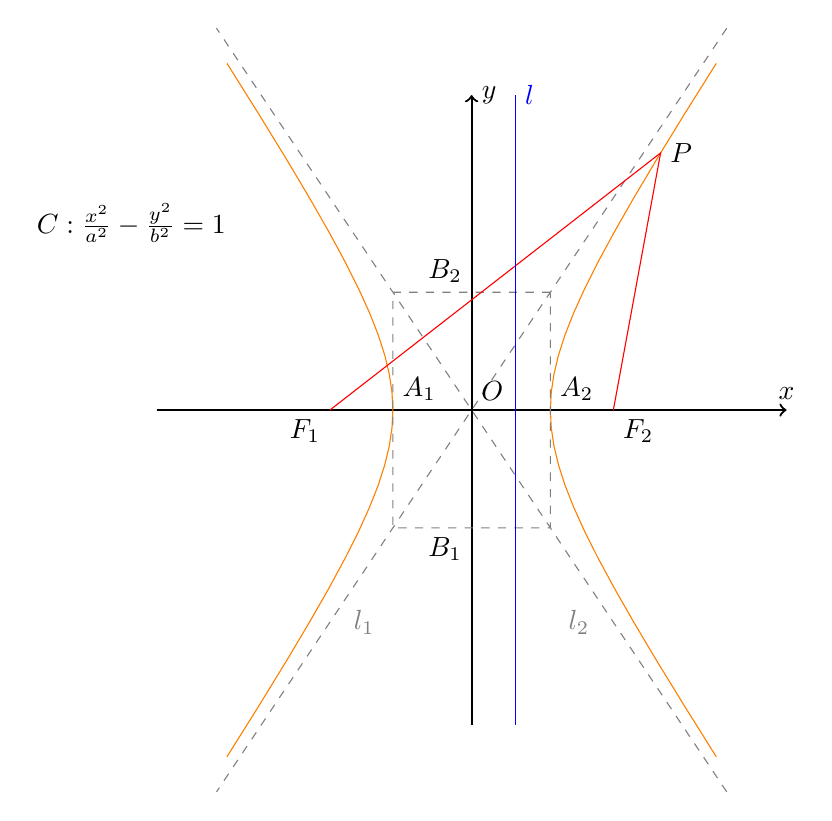
\begin{tikzpicture}
%\draw[gray,help lines,dashed] (-5,-3) grid (5,3);
\draw[thick,->] (-4,0) -- (4,0)node[above]{\(x\)};
\draw[thick,->] (0,-4) -- (0,4)node[right]{\(y\)};
\draw (-3,2)node[above left]{\(C: \frac{x^2}{a^2}-\frac{y^2}{b^2}=1\)};
\pgfmathsetmacro{\e}{1.8}   % eccentricity
\pgfmathsetmacro{\a}{1}
\pgfmathsetmacro{\b}{(\a*sqrt((\e)^2-1)}
\pgfmathsetmacro{\c}{(sqrt((\a)^2+(\b)^2))}
\pgfmathsetmacro{\px}{2.4}
\pgfmathsetmacro{\py}{sqrt(\b^2*(\px^2/\a^2-1))}
\pgfmathsetmacro{\d}{1.8} % 定义域
\draw[orange] plot[domain=-\d:\d] ({\a*cosh(\x)},{\b*sinh(\x)});
\draw[orange] plot[domain=-\d:\d] ({-\a*cosh(\x)},{\b*sinh(\x)});
\pgfmathsetmacro{\k}{1.8*\d}
\coordinate (F1) at (-\c,0);
\coordinate (F2) at (\c,0);
\coordinate (P) at (\px,\py);
\draw[gray,dashed] (\a,\b) -- (-\a,\b) -- (-\a,-\b) -- (\a,-\b) -- (\a,\b)
	(\k*\a,\k*\b) -- (-\k*\a,-\k*\b)
	(\k*\a,-\k*\b) -- (-\k*\a,\k*\b)
	(-\k*\a/2,-\k*\b/2)node[below right]{\(l_1\)}
	(\k*\a/2,-\k*\b/2)node[below left]{\(l_2\)};
\draw[red] (F1)node[below left,black]{\(F_1\)}
	-- (P)node[right,black]{\(P\)}
	-- (F2)node[below right,black]{\(F_2\)};
\pgfmathsetmacro{\dx}{\a^2/\c}
\draw[blue] (\dx,-4) -- (\dx,4)node[right]{\(l\)}; % 准线
\draw (0,0)node[above right]{\(O\)}
	(-\a,0)node[above right]{\(A_1\)}
	(\a,0)node[above right]{\(A_2\)}
	(0,-\b)node[below left]{\(B_1\)}
	(0,\b)node[above left]{\(B_2\)};
\end{tikzpicture}
\caption{双曲线的图形}
\label{figure:解析几何.双曲线的图形}
\end{figure}

我们根据双曲线的标准方程\begin{equation*}
\frac{x^2}{a^2} - \frac{y^2}{b^2} = 1
\end{equation*}来研究它的几何性质.
\begin{enumerate}
\item 范围

由标准方程可知,双曲线上的点的坐标\((x,y)\)都适合不等式\(\frac{x^2}{a^2}\geq1\),即\(x^2 \geq a^2\),所以\(x \geq a\)或\(x \leq -a\).这说明双曲线在两条直线\(x = \pm a\)的外侧.

\item 对称性

双曲线关于每条坐标轴和原点都是对称的.这时,坐标轴是双曲线的对称轴,原点是双曲线的对称中心.双曲线的对称中心叫做双曲线的\DefineConcept{中心}.

\item 顶点

在标准方程中,令\(y=0\),得\(x = \pm a\),因此双曲线和\(x\)轴有两个交点\(A_1(-a,0)\)、\(A_2(a,0)\).因为\(x\)轴是双曲线的对称轴,所以双曲线和它的对称轴有两个焦点,它们叫做双曲线的\DefineConcept{顶点}.

令\(x=0\),得\(y^2=-b^2\),这个方程没有实数根,说明双曲线和\(y\)轴没有交点,但我们也把\(B_1(0,-b)\)和\(B_2(0,b)\)画在\(y\)轴上.

线段\(A_1 A_2\)叫做双曲线的\DefineConcept{实轴},它的长等于\(2a\),\(a\)叫做双曲线的实半轴长.
线段\(B_1 B_2\)叫做双曲线的\DefineConcept{虚轴},它的长等于\(2b\),\(b\)叫做双曲线的虚半轴长.

\item 渐近线

经过\(A_2\)、\(A_1\)作\(y\)轴的平行线\(x = \pm a\),经过\(B_2\)、\(B_1\)作\(x\)轴的平行线\(y = \pm b\),四条直线围成一个矩形.矩形的两条对角线所在的直线是\(y = \pm\frac{b}{a}x\).可以看出,双曲线的各支向外延伸时,与这两条直线逐渐接近.我们把这两条直线叫做双曲线的\DefineConcept{渐近线}.

在方程\(\frac{x^2}{a^2}-\frac{y^2}{b^2}=1\)中,如果\(a=b\),那么双曲线方程为\(x^2-y^2=a^2\),它的实轴和虚轴的长都等于\(2a\).这时,四条直线\(x=\pm a\)、\(y=\pm a\)围成正方形;渐近线方程成为\(x=\pm y\),它们互相垂直,并且平分双曲线实轴与虚轴所成的角.像这样,实轴和虚轴等长的双曲线叫做\DefineConcept{等轴双曲线}.

\item 离心率

双曲线的焦距与实轴的比\(e = \frac{c}{a}\),叫做双曲线的\DefineConcept{离心率}.因为\(c > a\),所以双曲线的离心率\(e > 1\).

由等式\(c^2-a^2=b^2\)可得\begin{equation*}
\frac{b}{a} = \frac{\sqrt{c^2-b^2}}{a} = \sqrt{\frac{c^2}{a^2}-1} = \sqrt{e^2-1}.
\end{equation*}因此\(e\)越大,\(\frac{b}{a}\)也越大,即渐近线\(y = \pm\frac{b}{a}x\)的斜率的绝对值越大,这时双曲线的形状就从褊狭逐渐变得开阔.由此可知,双曲线的离心率越大,它的开口就越开阔.
\end{enumerate}

\begin{example}
以已知双曲线的虚轴为实轴,实轴为虚轴的双曲线叫做原双曲线的\DefineConcept{共轭双曲线}.求证:\begin{enumerate}
\item 双曲线和它的共轭双曲线有共同的渐近线;
\item 双曲线和它的共轭双曲线的四个焦点在同一个圆上.
\end{enumerate}
\begin{proof}
设已知双曲线的方程是\begin{equation*}
	\frac{x^2}{a^2}-\frac{y^2}{b^2}=1.
\end{equation*}
它的焦点坐标为\(F_1(-c,0)\)和\(F_2(c,0)\)
(\(c^2=a^2+b^2\)).
它的渐近线方程是\(y=\pm\frac{b}{a}x\).

根据定义,其共轭双曲线的方程是\begin{equation*}
\frac{y^2}{a^2}-\frac{x^2}{b^2}=1.
\end{equation*}它的交点坐标为\(F'_1(0,-c)\)和\(F'_2(0,c)\),
可见四个焦点都在圆\(x^2+y^2=c^2\)上.
它的共轭双曲线的渐近线方程是\(x=\pm\frac{a}{b}y\),
也即\(y=\pm\frac{b}{a}x\),
所以双曲线和它的共轭双曲线具有共同的渐近线.
\end{proof}
\end{example}

\begin{example}
点\(P(x,y)\)与定点\(F(c,0)\)的距离和它到定直线\(l: x = \frac{a^2}{c}\)的距离的比是常数\(\frac{c}{a}\)
(\(c > a > 0\)).
求点\(P\)的轨迹.
\begin{solution}
设点\(P\)到直线\(l\)的距离是\(d\),那么所求轨迹就是点集\begin{equation*}
\Set*{ P \given \frac{\abs{PF}}{d} = \frac{c}{a} },
\end{equation*}由此得\begin{equation*}
\frac{\sqrt{(x-c)^2+y^2}}{\abs{\frac{a^2}{c}-x}} = \frac{c}{a},
\end{equation*}化简得\begin{equation*}
(c^2-a^2)x^2 - a^2 y^2 = a^2(c^2-a^2).
\end{equation*}设\(b^2=c^2-a^2\),则可将上式进一步化简为\begin{equation*}
\frac{x^2}{a^2}-\frac{y^2}{b^2}=1.
\end{equation*}这是双曲线的标准方程,所以点\(P\)的轨迹是双曲线.
\end{solution}

由上例可知,点\(P\)与一个定点的距离和它到一条定直线的距离的比是常数
\(e = \frac{c}{a} > 1\)时,
这个点的轨迹是双曲线.
定点是双曲线的焦点,定直线叫做双曲线的\DefineConcept{准线},常数\(e\)是双曲线的离心率.

对于双曲线\(\frac{x^2}{a^2}-\frac{y^2}{b^2}=1\),相应于焦点\(F(c,0)\)的准线方程是\begin{equation*}
x = \frac{a^2}{c}
\quad\text{或}\quad
x = \frac{a}{e}.
\end{equation*}根据双曲线的对称性,相应于焦点\(F'(-c,0)\)的准线方程是\(x=-\frac{a^2}{c}\),所以双曲线有两条准线.
\end{example}

\begin{example}
证明:等轴双曲线的离心率是\(\sqrt2\).
\begin{proof}
由定义,等轴双曲线\(x^2-y^2=a^2\)的实半轴长与虚半轴长相等,即\(a=b>0\),故\(c^2 = a^2 + b^2 = 2 a^2\),\(c = \sqrt2 a\),那么等轴双曲线的离心率为\begin{equation*}
e = \frac{c}{a} = \frac{\sqrt2 a}{a} = \sqrt2.
\qedhere
\end{equation*}
\end{proof}
\end{example}

\begin{example}
证明:从双曲线的一个焦点到一条渐近线的距离等于虚半轴长.
\begin{proof}
设双曲线方程为\begin{equation*}
	\frac{x^2}{a^2}-\frac{y^2}{b^2}=1,
\end{equation*}
它的右焦点为\(F(c,0)\)
(\(c^2=a^2+b^2\)),
其中一条渐近线为\(y=\frac{b}{a}x\)或\(bx-ay=0\).
由点到直线的距离公式,焦点\(F\)到上述渐近线的距离为\begin{equation*}
	d = \frac{\abs{b \cdot c - a \cdot 0}}{\sqrt{b^2+(-a)^2}}
	= \frac{bc}{c} = b.
	\qedhere
\end{equation*}
\end{proof}
\end{example}

\begin{example}
已知双曲线\begin{equation*}
C: \frac{x^2}{a^2} - \frac{y^2}{b^2} = 1 \quad(a>b>1).
\end{equation*}求双曲线在其上任意一点\(P_0(x_0,y_0)\)处的切线方程.
\begin{solution}
因为点\(P_0(x_0,y_0)\)在双曲线\(C\)上,所以\begin{equation*}
\frac{x_0^2}{a^2} - \frac{y_0^2}{b^2} = 1
\quad\text{即}\quad
b^2 x_0^2 - a^2 y_0^2 = a^2 b^2.
\end{equation*}

当切线\(l\)与\(x\)轴相垂直时,显然只有\((-a,0)\)和\((a,0)\)两点可能是切点,
而它们各自的切线方程分别为\(x=-a\)和\(x=a\).

当切线\(l\)不与\(x\)轴相垂直时,
设切线方程为\(l: y = kx + p\),其中\(p = y_0 - k x_0\).
联立方程组,得\begin{equation*}
\begin{cases}
y = kx + p, \\
\frac{x^2}{a^2} - \frac{y^2}{b^2} = 1.
\end{cases}
\end{equation*}那么有\begin{equation*}
\frac{1}{a^2} x^2 - \frac{1}{b^2} (kx+p)^2 = 1,
\end{equation*}\begin{equation*}
b^2 x^2 - a^2 (k^2 x^2 + 2kpx + p^2) = a^2 b^2,
\end{equation*}\begin{equation*}
(b^2 - a^2 k^2) x^2 - 2 a^2 k p x - a^2 (p^2 + b^2) = 0.
\end{equation*}令判别式\(\Delta_1 = (2 a^2 k p)^2 + 4 (b^2 - a^2 k^2) a^2 (p^2 + b^2) = 0\),得\begin{equation*}
4 a^4 k^2 p^2 = 4 (a^2 k^2 - b^2) a^2 (p^2 + b^2),
\end{equation*}\begin{equation*}
a^2 k^2 p^2 = (a^2 k^2 - b^2)(p^2 + b^2),
\end{equation*}\begin{equation*}
a^2 b^2 k^2 = b^2(p^2 + b^2),
\end{equation*}\begin{equation*}
a^2 k^2 = p^2 + b^2,
\end{equation*}
代入\(p = y_0 - k x_0\),得\begin{equation*}
a^2 k^2 = (y_0 - k x_0)^2 + b^2,
\end{equation*}\begin{equation*}
y_0^2 - 2k x_0 y_0 + k^2 x_0^2 + b^2 = a^2 k^2,
\end{equation*}\begin{equation*}
(x_0^2 - a^2) k^2 - 2 x_0 y_0 k + (y_0^2 + b^2) = 0.
\end{equation*}上式的判别式\(\Delta_2 = (2 x_0 y_0)^2 - 4(x_0^2 - a^2)(y_0^2 + b^2)
= 4(a^2 b^2 + a^2 y_0^2 - b^2 x_0^2) = 0\),故可解得\begin{equation*}
k = \frac{2 x_0 y_0}{2 (x_0^2 - a^2)}
= \frac{x_0 y_0}{x_0^2 - a^2}.
\end{equation*}那么\(l\)的方程为\begin{equation*}
y - y_0 = \frac{x_0 y_0}{x_0^2 - a^2} (x - x_0),
\end{equation*}\begin{equation*}
(x_0^2 - a^2) y = x_0 y_0 x + (x_0^2 - a^2) y_0 - x_0^2 y_0
= x_0 y_0 x - a^2 y_0,
\end{equation*}\begin{equation*}
x_0 y_0 x + (a^2 - x_0^2) y = a^2 y_0,
\end{equation*}\begin{equation*}
\frac{x_0 x}{a^2} + (a^2 - x_0^2) \frac{y_0 y}{a^2 y_0^2} = 1,
\end{equation*}\begin{equation*}
\frac{x_0 x}{a^2} + (a^2 - x_0^2) \frac{y_0 y}{(x_0^2 - a^2) b^2} = 1,
\end{equation*}最后化简得\begin{equation}\label{equation:解析几何.双曲线的切线}
\frac{x_0 x}{a^2} - \frac{y_0 y}{b^2} = 1.
\end{equation}
这就是双曲线在其上任意一点\(P_0(x_0,y_0)\)处的切线方程.
\end{solution}
\end{example}

\begin{theorem}[双曲线的焦点三角形]
设\(P\)是双曲线\(C: \frac{x^2}{a^2} - \frac{y^2}{b^2} = 1\ (a>0,b>0)\)上任一点,
\(F_1\)、\(F_2\)是\(C\)的焦点,那么\begin{equation*}
S_{\triangle P F_1 F_2} = \frac{b^2}{\tan(\theta/2)},
\end{equation*}其中\(\theta=\angle{F_1 P F_2}\).
\end{theorem}

\subsection{抛物线}
在平面内取一条曲线,
如果这条曲线上的任意一点到某条定直线的距离,
和它到某个定点的距离相等,
就把这条曲线叫做\DefineConcept{抛物线}(parabola).
这个定点叫做这条抛物线的\DefineConcept{焦点}.
这条定直线叫做这条抛物线的\DefineConcept{准线}.

取经过焦点\(F\)且垂直于准线\(l\)的直线为\(x\)轴,
\(x\)轴于\(l\)相交于点\(K\),
以线段\(KF\)的垂直平分线为\(y\)轴.
设\(\abs{KF}=p\),
那么,焦点\(F\)的坐标为\((\frac{p}{2},0)\),
准线\(l\)的方程为\(x=-\frac{p}{2}\).

设抛物线上的点\(P(x,y)\)到\(l\)的距离为\(d(P)\).
抛物线就是点集\begin{equation*}
	\Set*{ P \given \abs{PF} = d(P) }.
\end{equation*}
因为\(\abs{PF} = \sqrt{\left(x-\frac{p}{2}\right)^2+y^2}\),
\(d = \abs{x+\frac{p}{2}}\),
所以\begin{equation*}
	\sqrt{\left(x-\frac{p}{2}\right)^2+y^2} = \abs{x+\frac{p}{2}}.
\end{equation*}
将上式两边平方,并化简得\begin{equation}
	y^2 = 2px, \quad p > 0.
\end{equation}
这个方程叫做\DefineConcept{抛物线的标准方程},它所表示的抛物线的焦点在\(x\)轴的正半轴上,
坐标是\((\frac{p}{2},0)\),准线方程是\(x=-\frac{p}{2}\).

一条抛物线,由于它在坐标平面上的位置不同,方程也不同,
所以抛物线的标准方程还有其他几种形式:\begin{gather}
	y^2 = -2px, \\
	x^2 = 2py, \\
	x^2 = -2py.
\end{gather}

\begin{figure}[htb]
\centering
\begin{tikzpicture}
%\draw[gray,help lines,dashed] (-3,-3) grid (3,3);
\draw[thick,->] (-3,0) -> (4,0)node[above]{\(x\)};
\draw[thick,->] (0,-4) -> (0,4)node[right]{\(y\)};
\draw (0,0)node[below left]{\(O\)};
\pgfmathsetmacro{\p}{2}
\pgfmathsetmacro{\x}{3}
\pgfmathsetmacro{\y}{sqrt(2*\p*\x)}
\pgfmathsetmacro{\f}{\p/2}
\coordinate (F)at(\f,0);
\draw[orange] [rotate=-90](0,0)parabola(\y,\x) [rotate=180](0,0)parabola(\y,-\x);
\draw[purple] (-\f,-4)--(-\f,4);
\draw (2,2)node[above right]{\(C: y^2 = 2px\ (p>0)\)}
	(-\f,-1)node[below left]{\(l: x = -\frac{p}{2}\)};
\fill (F)circle(2pt)node[below right]{\(F\)};
\pgfmathsetmacro{\px}{\f/2}
\pgfmathsetmacro{\py}{\p/sqrt(2)}
\coordinate (P)at(\px,\py);
\coordinate (Q)at(-\f,\py);
\coordinate (K)at(-\f,0);
\draw[red] (F)--(P)node[above,black]{\(P\)}--(Q)node[left,black]{\(Q\)}
	pic[draw=gray,-,angle radius=0.3cm]{right angle=P--Q--K};
\draw (K)node[below left]{\(K\)};
\coordinate (M)at(\f,\p);
\coordinate (N)at(\f,-\p);
\draw[blue] (M)node[above,black]{\(M\)}--(N)node[below,black]{\(N\)}
	pic[draw=gray,-,angle radius=0.3cm]{right angle=N--F--K};
\end{tikzpicture}
\caption{抛物线的图形}
\label{figure:解析几何.抛物线的图形}
\end{figure}

我们根据抛物线的标准方程\begin{equation*}
y^2 = 2px, \quad p > 0
\end{equation*}来研究它的几何性质.
\begin{enumerate}
\item 范围

因为\(p>0\),由标准方程可知,抛物线上的点的坐标\((x,y)\)都适合不等式\(x \geq 0\),所以这条抛物线在\(y\)轴的右侧.当\(x\)的值增大时,\(\abs{y}\)也增大,这说明抛物线向右上方和右下方无限延伸.

\item 对称性

以\(-y\)代\(y\),标准方程形式不变,所以这个抛物线关于\(x\)轴对称,我们把抛物线的对称轴叫做抛物线的\DefineConcept{轴}.

\item 顶点

抛物线和它的轴的交点叫做抛物线的\DefineConcept{顶点}.
在标准方程中,当\(y=0\)时,\(x=0\),因此标准方程所表示的抛物线的顶点就是坐标原点.
焦点到顶点的距离,称为抛物线的\DefineConcept{焦距}.

\item 离心率

抛物线上的点\(P\)与焦点和准线的距离的比,叫做抛物线的\DefineConcept{离心率},用\(e\)表示.
由抛物线的定义,抛物线的离心率为\(e = 1\).
\end{enumerate}

\begin{example}
已知抛物线方程\(C: y^2=2px\ (p>0)\).
下面讨论过焦点\(F(p/2,0)\)的直线\(l\)与抛物线的交点个数.
\begin{enumerate}
	\item 当直线\(l\)的方程为\(y=0\)时,
	代入抛物线方程得\(2px = 0\),解得\(x=0\).
	可见直线\(l\)与抛物线\(C\)只有一个交点,即坐标原点\(O\).

	\item 当直线\(l\)的方程为\(x=p/2\)时,
	代入抛物线方程得\(y^2=2p\cdot(p/2)=p^2\),解得\(y=\pm p\).
	可见直线\(l\)与抛物线\(C\)有两个交点\(P(p/2,p)\)和\(Q(p/2,-p)\).
	焦点弦长为\(\abs{PQ} = 2p\).

	\begin{center}
		\begin{tikzpicture}
			%\draw[gray,help lines,dashed] (-3,-3) grid (3,3);
			\draw[thick,->] (-2,0) -> (4,0)node[above]{\(x\)};
			\draw[thick,->] (0,-4) -> (0,4)node[right]{\(y\)};
			\draw (0,0)node[below left]{\(O\)};
			\pgfmathsetmacro{\p}{2}  % 参数p
			\pgfmathsetmacro{\x}{3}
			\pgfmathsetmacro{\y}{sqrt(2*\p*\x)}
			\pgfmathsetmacro{\f}{\p/2}  % 焦点横坐标
			\coordinate (F)at(\f,0);
			\coordinate (2F)at(2\f,0);
			\draw[orange] [rotate=-90](0,0)parabola(\y,\x) [rotate=180](0,0)parabola(\y,-\x);
			\draw[purple] (-\f,-4)--(-\f,4); % 准线
			\draw (2,-3)node[above right]{\(C: y^2 = 2px\ (p>0)\)};
			\pgfmathsetmacro{\k}{3}  % 焦点弦 斜率
			\pgfmathsetmacro{\a}{\p/(2*\k^2)}
			\pgfmathsetmacro{\b}{\p/\k}
			\pgfmathsetmacro{\c}{sqrt(\k^2+1)}
			\pgfmathsetmacro{\px}{\a*(\c+1)^2}
			\pgfmathsetmacro{\py}{\b*(\c+1)}
			\pgfmathsetmacro{\qx}{\a*(\c-1)^2}
			\pgfmathsetmacro{\qy}{-\b*(\c-1)}
			\coordinate (P)at(\px,\py);
			\coordinate (Q)at(\qx,\qy);
			\coordinate (P1)at(-\f,\py);
			\coordinate (Q1)at(-\f,\qy);
			\coordinate (K)at(-\f,0);
			\fill (P)circle(2pt)node[below right]{\(P\)}
				(F)circle(2pt)node[below right]{\(F\)}
				(Q)circle(2pt)node[right]{\(Q\)};
			\draw[red] (P)--(P1)node[left,black]{\(P_1\)}
				pic[draw=gray,-,angle radius=0.3cm]{right angle=P--P1--K}
				(Q)--(Q1)node[left,black]{\(Q_1\)}
				pic[draw=gray,-,angle radius=0.3cm]{right angle=Q--Q1--K};
			\draw[blue] (P)--(F)--(Q);
			\draw pic["\(\theta\)",draw=gray,-,angle eccentricity=1.7,angle radius=5mm]{angle=2F--F--P};
		\end{tikzpicture}
	\end{center}

	\item 当直线\(l\)的方程为\(y=k\left(x-\frac{p}{2}\right)\ (k\neq0)\)时,代入抛物线方程得\begin{equation*}
		\left[k \left(x-\frac{p}{2}\right)\right]^2 = 2px,
	\end{equation*}
	化简得\begin{gather}
		k^2 x^2 - (k^2 + 2)px + \frac{1}{4} k^2 p^2 = 0, \tag1
	\end{gather}
	因为这个关于\(x\)的一元二次方程的判别式为\begin{equation*}
		\Delta = [- (k^2 + 2)p]^2 - 4 \cdot k^2 \cdot \frac{1}{4} k^2 p^2
		= 4 p^2 (k^2 + 1) > 0,
	\end{equation*}
	所以(1)式总有两个实根\begin{equation*}
		x_{1,2} = \frac{(k^2+2)p \pm \sqrt\Delta}{2 k^2}
		= \frac{p}{2 k^2} (\sqrt{k^2+1} \pm 1)^2.
	\end{equation*}
	可见直线\(l\)与抛物线\(C\)有两个交点\(P(x_1,y_1)\)和\(Q(x_2,y_2)\).
	不妨设\(x_1 > x_2\),即\begin{equation*}
		x_1 = \frac{(k^2+2)p + \sqrt\Delta}{2 k^2}
		= \frac{p}{2 k^2} (\sqrt{k^2+1} + 1)^2,
	\end{equation*}\begin{equation*}
		x_2 = \frac{(k^2+2)p - \sqrt\Delta}{2 k^2}
		= \frac{p}{2 k^2} (\sqrt{k^2+1} - 1)^2.
	\end{equation*}
	将\(x_{1,2}\)代入抛物线方程得\begin{equation*}
		y^2 = 2 p^2 \frac{(\sqrt{k^2+1}\pm1)^2}{2 k^2}
		= \frac{p^2}{k^2} (\sqrt{k^2+1}\pm1)^2,
	\end{equation*}\begin{equation*}
		y = \pm \frac{p}{k} (\sqrt{k^2+1}\pm1).
	\end{equation*}
	当\(k>0\)时,由\(x_1 > x_2\)可知\(y_1 > 0 > y_2\),那么\begin{equation*}
		y_1 = \frac{p}{k} (\sqrt{k^2+1}+1),
		\qquad
		y_2 = -\frac{p}{k} (\sqrt{k^2+1}-1).
	\end{equation*}
	由两点间距离公式,焦点弦长为\begin{equation}
		\abs{PQ} = \sqrt{
		\left(\frac{p}{2 k^2} \cdot 4 \sqrt{k^2+1}\right)^2
		+\left(\frac{p}{k} \cdot 2 \sqrt{k^2+1}\right)^2
		} = 2p \left(1+\frac{1}{k^2}\right).
	\end{equation}
	若记\(k=\tan\theta\),则上述弦长公式也可改写为\begin{equation}
		\abs{PQ} = 2p \frac{\tan^2\theta+1}{\tan^2\theta}
		= 2p \frac{\sec^2\theta}{\tan^2\theta}
		= 2p \frac{1}{\sin^2\theta}
		= 2p \csc^2\theta.
	\end{equation}

	现在我们来检验上述弦长公式的正确性.
	根据抛物线的定义,抛物线上一点到焦点与其到准线的距离相等,
	故\(\abs{PF} = \abs{P P_1} = x_1 + \frac{p}{2}\),
	\(\abs{QF} = \abs{Q Q_1} = x_2 + \frac{p}{2}\),
	那么\(\abs{PQ} = \abs{PF}+\abs{QF} = x_1 + x_2 + p\).
	代入\(x_{1,2}\),得\begin{align*}
		\abs{PQ} &= \frac{p}{2 k^2} \left[(\sqrt{k^2+1} + 1)^2 + (\sqrt{k^2+1} - 1)^2\right] + p \\
		&= p\left[\frac{2(k^2 + 1) + 2}{2 k^2} + 1\right]
		= p \frac{4k^2 + 4}{2k^2}
		= 2p \left(1+\frac{1}{k^2}\right).
	\end{align*}
\end{enumerate}

另外,可以注意到,\(P\)、\(Q\)两点的坐标满足\begin{equation}
	x_1 \cdot x_2 = \frac{p^2}{4},
	\qquad
	y_1 \cdot y_2 = -p^2.
\end{equation}

\(P\)、\(Q\)两点的焦半径\(\abs{FP}\)、\(\abs{FQ}\)满足\begin{equation}
	\frac{1}{\abs{FP}} + \frac{1}{\abs{FB}}
	= \frac{2}{p}.
\end{equation}
\end{example}

\subsection{平面曲线在极坐标系下方程}
在平面内取一个定点\(O\),称为\DefineConcept{极点}.
过极点引一条射线\(Ox\),称为\DefineConcept{极轴}.
再选一个长度单位和计算角度的正方向(通常取逆时针方向),
这样的坐标系称为\DefineConcept{极坐标系}.
连接平面内任意一点\(P\)与极点\(O\)所得的线段\(OP\),称为“点\(P\)的\DefineConcept{极径}”.
这条线段\(OP\)与极轴所得的夹角\(\angle POx\),称为“点\(P\)的\DefineConcept{极角}”.

\begin{table}[htb]
	\centering
	\begin{tblr}{c|c|c}
		\hline
		& 直角坐标方程
		& 极坐标方程 \\ \hline
		过极点的直线的方程
			& \(y = x \tan\theta_0\)
			& \(\theta=\theta_0\ (\text{$\theta_0$是常数})\) \\
		垂直于极轴的直线的方程
			& \(x = a\)
			& \(\rho\cos\theta=a\) \\
		平行于极轴的直线的方程
			& \(y = a\)
			& \(\rho\sin\theta=a\) \\
			& \(x + y = a\)
			& \(\rho = \frac{a}{\cos\theta + \sin\theta}\) \\
		中心在极点、半径为\(r\)的圆
			& \(x^2+y^2=r^2\)
			& \(\rho=r\) \\
		中心在\((r,0)\)、半径为\(r\)的圆
			& \((x-r)^2+y^2=r^2\)
			& \(\rho=2r\cos\theta\) \\
		中心在\((r,\pi)\)、半径为\(r\)的圆
			& \((x+r)^2+y^2=r^2\)
			& \(\rho=-2r\cos\theta\) \\
		中心在\((\rho_0,\theta_0)\)、半径为\(r\)的圆
			&
			& \(\rho^2+\rho_0^2-2\rho_0\rho\cos(\theta-\theta_0)=r^2\) \\
		\hline
	\end{tblr}
	\caption{}
\end{table}


\section{本章总结}
\subsection*{向量及其运算}
\begin{table}[htb]
	\centering
	\begin{tabular}{|c|c|c|c|}
	\hline
	\multicolumn{2}{|c|}{加法} & \multicolumn{2}{c|}{数乘} \\ \hline
	交换律 & \(\vb{a}+\vb{b}=\vb{b}+\vb{a}\) &
		结合律 & \(\lambda(\mu\vb{a})=\mu(\lambda\vb{a})=(\lambda\mu)\vb{a}\) \\ \hline
	\multirow{2}{*}{结合律} & \multirow{2}{*}{\((\vb{a}+\vb{b})+\vb{c}=\vb{a}+(\vb{b}+\vb{c})\)} &
		\multirow{2}{*}{分配律} & \((\lambda+\mu)\vb{a}=\lambda\vb{a}+\mu\vb{a}\) \\
	 & & & \(\lambda(\vb{a}+\vb{b})=\lambda\vb{a}+\lambda\vb{b}\) \\ \hline
	\multicolumn{2}{|c|}{点乘} & \multicolumn{2}{c|}{叉乘} \\ \hline
	交换律 & \(\VectorInnerProductDot{\vb{a}}{\vb{b}}=\VectorInnerProductDot{\vb{b}}{\vb{a}}\) &
		负交换律 & \(\VectorOuterProduct{\vb{a}}{\vb{b}}=-\VectorOuterProduct{\vb{b}}{\vb{a}}\) \\ \hline
	分配律 & \(\VectorInnerProductDot{(\vb{a}+\vb{b})}{\vb{c}}=\VectorInnerProductDot{\vb{a}}{\vb{c}}+\VectorInnerProductDot{\vb{b}}{\vb{c}}\) &
		分配律 & \(\VectorOuterProduct{(\vb{a}+\vb{b})}{\vb{c}}=\VectorOuterProduct{\vb{a}}{\vb{c}}+\VectorOuterProduct{\vb{b}}{\vb{c}}\) \\ \hline
	\multirow{3}{*}{结合律} & \(\VectorInnerProductDot{(\lambda\vb{a})}{\vb{b}}=\lambda(\VectorInnerProductDot{\vb{a}}{\vb{b}})\) & \multirow{3}{*}{结合律} & \multirow{3}{*}{\(\VectorOuterProduct{(\lambda\vb{a})}{\vb{b}}=\VectorOuterProduct{\vb{a}}{(\lambda\vb{b})}=\lambda(\VectorOuterProduct{\vb{a}}{\vb{b}})\)} \\
		& \(\VectorInnerProductDot{\vb{a}}{(\lambda\vb{b})}=\lambda(\VectorInnerProductDot{\vb{a}}{\vb{b}})\) & & \\
		& \(\VectorInnerProductDot{(\lambda\vb{a})}{(\mu\vb{b})}=\lambda\mu(\VectorInnerProductDot{\vb{a}}{\vb{b}})\) & & \\
	\hline
	\end{tabular}
	\caption{向量的运算法则}
\end{table}

\subsection*{常见的坐标系}
极坐标系是一种平面坐标系.
极坐标系上的点\((\rho,\theta)\)与平面直角坐标系上的点\((x,y)\)存在以下的一一对应关系:\begin{equation*}
\left\{ \begin{array}{l}
x = \rho\cos\theta, \\
y = \rho\sin\theta. \\
\end{array} \right.
\end{equation*}

柱面坐标系是一种空间坐标系.
柱面坐标系上的点\((\rho,\theta,z)\)与空间直角坐标系上的点\((x,y,z)\)存在以下的一一对应关系:\begin{equation*}
\left\{ \begin{array}{l}
x = \rho\cos\theta, \\
y = \rho\sin\theta, \\
z = z. \\
\end{array} \right.
\end{equation*}

球极坐标系是一种空间坐标系.
球极坐标系上的点\((r,\theta,\phi)\)与空间直角坐标系上的点\((x,y,z)\)存在以下的一一对应关系:\begin{equation*}
\left\{ \begin{array}{l}
x = r \sin\phi \cos\theta, \\
y = r \sin\phi \sin\theta, \\
z = r \cos\phi. \\
\end{array} \right.
\end{equation*}

\begin{figure}[h]
	\centering
	\begin{tikzpicture}
		\coordinate (O) at (0,0);
		\coordinate (M) at (2,2);
		\coordinate (P) at (2,-1.2);
		\coordinate (A) at (-0.8,-1.2);
		\coordinate (Z) at (0,1);
		\draw (O)node[left]{\(O\)}
				-- (M)node[right]{\(M\)} node[midway,above]{\(r\)}
				-- (P)node[right]{\(P\)} node[midway,right]{\(z\)}
				-- (A)node[left]{\(A\)} node[midway,below]{\(y\)}
				-- (O)node[midway,left]{\(x\)}
			(O) -- (P)
			pic["\(\phi\)",draw=orange,<-,angle eccentricity=1.3,angle radius=0.6cm]{angle=M--O--Z}
			pic["\(\theta\)",draw=orange,->,angle eccentricity=1.5,angle radius=0.4cm]{angle=A--O--P};
		\begin{scope}[>=Stealth,->,ultra thick]
			\draw(0,0) -- (-1.5,-2.25) node[right]{\(x\)};
			\draw(0,0) -- (3,0) node[right]{\(y\)};
			\draw(0,0) -- (0,3) node[above]{\(z\)};
		\end{scope}
	\end{tikzpicture}
	\caption{球极坐标系}
\end{figure}
